\documentclass{exam}
\usepackage[utf8]{inputenc}
\usepackage{lmodern}
\usepackage{microtype}

% \usepackage[parfill]{parskip}
\usepackage[dvipsnames]{xcolor}
\usepackage{amsmath}
\usepackage{amsfonts}
\usepackage{amsthm}
\usepackage{siunitx}
\DeclareSIUnit\year{yr}
\DeclareSIUnit\foot{ft}
\DeclareSIUnit\litre{\liter}

\usepackage{skull}

\usepackage{pgfplots}
\usepgfplotslibrary{polar}
\pgfplotsset{compat=1.11}
\usepgfplotslibrary{statistics}
\usepackage{graphicx}
\usepackage{sidecap}
\sidecaptionvpos{figure}{c}
\usepackage{float}
\usepackage{gensymb}
\usepackage{tkz-euclide}
\usetkzobj{all}
\usepackage{commath}
\usepackage{hyperref}
\usepackage{enumitem}
\usepackage{wasysym}
\usepackage{multicol}
\usepackage{mathtools}
\usepackage{tcolorbox}
\usepackage{tabularx}
\usepackage[version=4]{mhchem}
\usepackage{changepage}
\usepackage{listings}
\lstset{basicstyle=\ttfamily\linespread{0.8}\small}

\renewcommand*{\thefootnote}{\fnsymbol{footnote}}

\newtheorem*{thm}{Theorem}
\newtheorem*{iden}{Identity}
\newtheorem*{lemma}{Lemma}
\newtheorem{obs}{Observation}
\theoremstyle{definition}
\newtheorem*{defn}{Definition}
\newtheorem*{ex}{Example}
\newtheorem{con}{Construction}
\newtheorem*{alg}{Algorithm}

\newtheoremstyle{break}
  {\topsep}{\topsep}%
  {\itshape}{}%
  {\bfseries}{}%
  {\newline}{}%
\theoremstyle{break}
\newtheorem*{bthm}{Theorem}

% russian integral
\usepackage{scalerel}
\DeclareMathOperator*{\rint}{\scalerel*{\rotatebox{17}{$\!\int\!$}}{\int}}

% \DeclareMathOperator*{\rint}{\int}

\pgfplotsset{vasymptote/.style={
    before end axis/.append code={
        \draw[densely dashed] ({rel axis cs:0,0} -| {axis cs:#1,0})
        -- ({rel axis cs:0,1} -| {axis cs:#1,0});
    }
}}

% \pointsinrightmargin
\boxedpoints
\pointname{}

\newcommand{\questioA}{\question[\texttt{\textbf{\color{Cerulean} A}}]}
\newcommand{\questioM}{\question[\texttt{\textbf{\color{PineGreen} M}}]}
\newcommand{\questioE}{\question[\texttt{\textbf{\color{WildStrawberry} E}}]}
\newcommand{\questioS}{\question[\texttt{\textbf{\color{Goldenrod} S}}]}
\newcommand{\questioO}{\question[\texttt{\textbf{\color{BurntOrange} O}}]}

\newcommand{\parA}{\part[\texttt{\textbf{\color{Cerulean} A}}]}
\newcommand{\parM}{\part[\texttt{\textbf{\color{PineGreen} M}}]}
\newcommand{\parE}{\part[\texttt{\textbf{\color{WildStrawberry} E}}]}
\newcommand{\parS}{\part[\texttt{\textbf{\color{Goldenrod} S}}]}
\newcommand{\parO}{\part[\texttt{\textbf{\color{BurntOrange} O}}]}

\newcommand{\subparA}{\subpart[\texttt{\textbf{\color{Cerulean} A}}]}
\newcommand{\subparM}{\subpart[\texttt{\textbf{\color{PineGreen} M}}]}
\newcommand{\subparE}{\subpart[\texttt{\textbf{\color{WildStrawberry} E}}]}
\newcommand{\subparS}{\subpart[\texttt{\textbf{\color{Goldenrod} S}}]}
\newcommand{\subparO}{\subpart[\texttt{\textbf{\color{BurntOrange} O}}]}

\newcommand{\mainHeader}[2]{\section*{NCEA Level 2 Mathematics\\#1. #2}}
\newcommand{\mainHeaderHw}[2]{\section*{NCEA Level 2 Mathematics (Homework)\\#1. #2}}
\newcommand{\seealso}[1]{\begin{center}\emph{See also #1.}\end{center}}
\newcommand{\drills}[1]{\begin{center}\emph{Drill problems: #1.}\end{center}}
\newcommand{\basedon}[1]{\begin{center}\emph{Notes largely based on #1.}\end{center}}


\begin{document}

\mainHeaderHw{12}{Tangent Lines and Approximations}
\subsection*{Reading}
So far, we have only looked at `nice' functions. However, it is possible to find functions which are not
so nice, in the sense that the derivative does not exist at some point. What does this mean? It means that
at some point, the graph of the function doesn't have a well-defined slope. For example, the function could
become vertical (what is the slope of a vertical line?), or it could jump from one place to another without
passing any of the points in between. Note that a function can be differentiable everywhere except one point,
for example the absolute value function! Here are some examples of some non-differentiable functions.

\begin{figure}[h]
  \begin{minipage}{0.5\textwidth}
  \begin{center}
    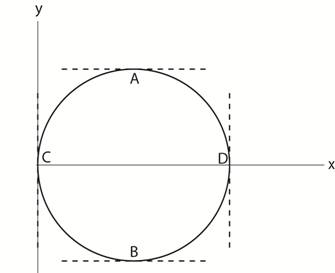
\includegraphics[height=120px]{circle}\\
    \small{The circle is not differentiable at $ C $ or $ D $ because the tangent lines are vertical.}
  \end{center}
  \end{minipage}
  \begin{minipage}{0.5\textwidth}
  \begin{center}
    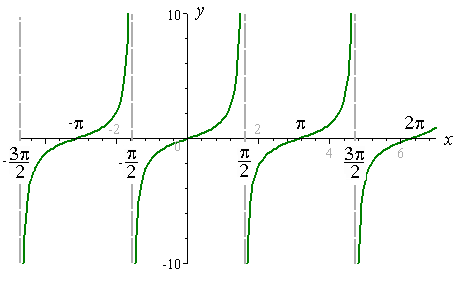
\includegraphics[height=120px]{tan}\\
    \small{The $ \tan $ function is not differentiable when the angle is an odd multiple of $ \frac{\pi}{2} $ because the function is undefined there.}
  \end{center}
  \end{minipage}
  \begin{minipage}{0.5\textwidth}
  \begin{center}
    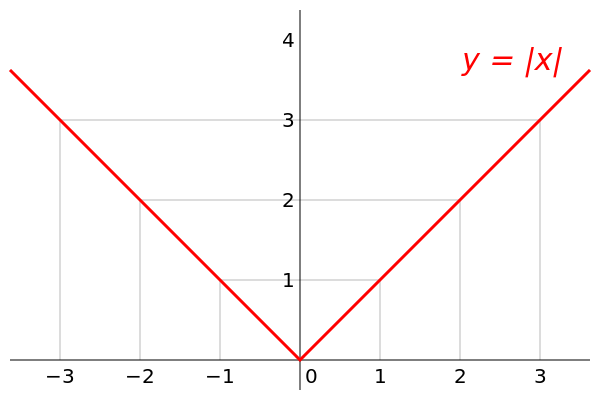
\includegraphics[height=120px]{abs}\\
    \small{The absolute value function is not differentiable at $ x = 0 $ because it has no tangent line (try to draw one in!).}
  \end{center}
  \end{minipage}
  \begin{minipage}{0.5\textwidth}
  \begin{center}
    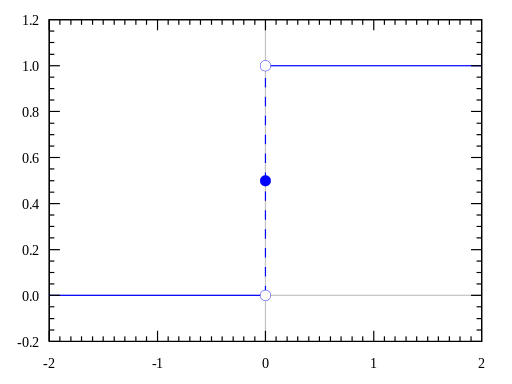
\includegraphics[height=120px]{heaviside}\\
    \small{The Heaviside step function is the derivative of the absolute value (can you see this geometrically?) with $ H(0) = \frac{1}{2} $, plugging
           the hole. However, because it is not continuous it is not differentiable at $ x = 0 $.}
  \end{center}
  \end{minipage}
  \begin{minipage}{\textwidth}
  \begin{center}
    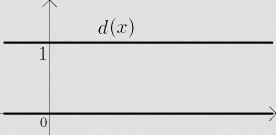
\includegraphics[height=80px]{dirichlet}\\
    \small{The Dirichlet function $ d(x) $ takes the value 1 when $ x $ is irrational and 0 when $ x $ is rational, and so is continuous nowhere
           (there is a rational number between any two irrationals and vice versa, so the function jumps between 0 and 1 infinitely often). As you
           might expect, it is differentiable nowhere.}
  \end{center}
  \end{minipage}
\end{figure}

\clearpage
\subsection*{Questions}
\begin{questions}
  \question A function $ f $ is given by
            \begin{equation}
              f(x) = 2 - 4x + 5x^2 + ax^3.
            \end{equation}
            The gradient of the graph at the point where $ x = 1 $ is 3. Find the value of $ a $.
  \question Give the equation of the tangent line to the curve
            \begin{displaymath}
              y = 3x^3 - \sqrt{x} + \frac{1}{x^3}
            \end{displaymath}
            at the point $ (1, 3) $.
  \question Use calculus to show that the line $ y = 15x - 12 $ is tangent to the graph of the function $ f(x) = 4x^2 - x + 4 $.
\end{questions}

\end{document}
